\chapter{Signal and background modelling}
\label{chap:s_b_modelling}

\section{Introduction}

In order to extract a potential \Hee signal, a maximum likelihood fit to the observed \mee distribution in data is performed. To estimate the expected mass distributions, a parameterisation of both the signal and background components of the \mee spectrum is required. Once constructed, the parameters describing the models are chosen such that the value of twice the negative logarithm of the likelihood (2NLL) is minimised. 

Signal models are derived from simulated samples, for a selection of Higgs boson mass hypotheses. The dependence on \mH is built into the shape parameters and overall normalisation of the signal yield. Conversely, background modelling uses a data-driven approach, where a set of candidate models are constructed by fitting to sideband regions of the \mee distribution. All candidate functions fitting well are considered when extracting the final results, in a procedure known as the discrete profiling method~\cite{envelope_method}. The method is similar to that used in many previous SM \Hgg analyses~\cite{HIG-16-040,HIG-18-029,HIG-19-015} by the CMS collaboration, where it has been extensively validated.

When extracting the analysis' results, a set of systematic uncertainties are included to account for imperfect descriptions of the analysis inputs. These uncertainties, which are divided into theoretical and experimental sources, are implemented using nuisance parameters. While not being of interest themselves, nuisance parameters are allowed to modify the extracted parameter(s) of interest during the final fit. The analysis uses both continuous and discrete nuisance parameters to implement systematic uncertainties.

This chapter describes the strategy used to construct models for signal and background events, with the formalisation of the likelihood fit left to chapter~\ref{chap:results}. A description of all theoretical and experimental systematic uncertainties is also given, including the magnitude of their effect.

\section{Signal modelling}
\label{sec:hee_s_modelling}

In this analysis, models of the \mee distribution for \Hee signal processes are built using simulated samples. An independent model is constructed for each signal process contributing to each analysis category. Models are also constructed separately for each year of data taking, to account for any per-year differences in the CMS detector response and performance. In total, this results in $72$ models (4 signal processes $\times$ 6 analysis categories $\times$ 3 years). 

Each signal model is constructed as a sum of up to five Gaussian probability distributions. Four of the five Gaussians are used to model the core of the \mee distribution, where the majority of events lie, while the fifth is included to account for the lower tail in \mee, resulting from final-state radiation (FSR). The mean of this so-called FSR Gaussian is centred at lower masses with respect to the nominal set and has larger width, to model the extended tail. Alternative signal parameterisations are also tested, namely Double Crystal Ball functions~\cite{DCB}. The resulting signal models are similar to those produced with the nominal strategy; hence, the more simple approach of summing Gaussian probability distributions is kept. Figure~\ref{fig:smode_components} shows the shape components of the signal models for \ggH signal entering the highest $S/B$ category targeting \ggH events in 2017, and similarly for VBF signal entering the purest category targeting VBF events, at a nominal Higgs boson mass of 125~GeV. 

%The affect of including the additional Gaussian on the expected limit is, however, small, resulting in changes of less than 1\% per analysis category.

\begin{figure}[htbp!]
\centering
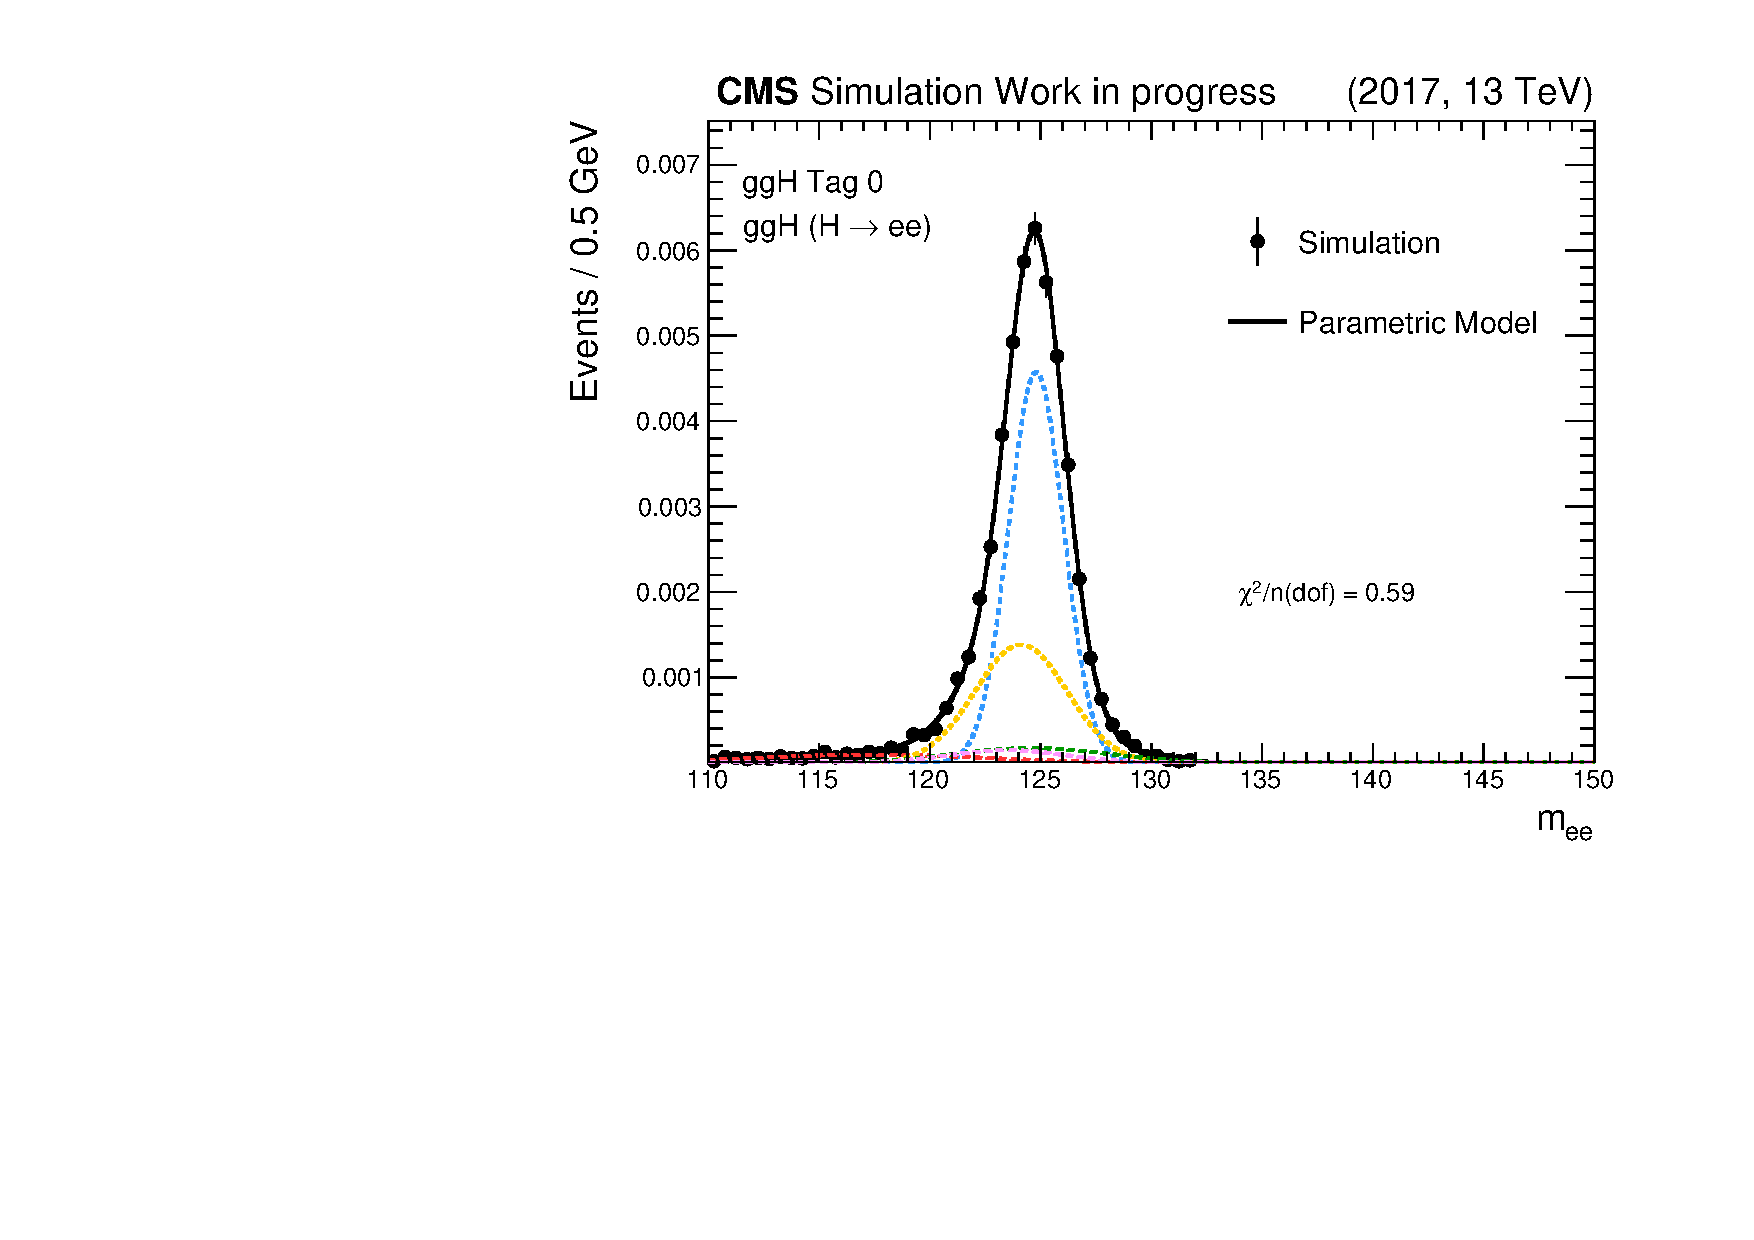
\includegraphics[width =0.49\linewidth]{Figures/Hee/Results/sigModels/GaussSums/total_shape_pdf_components_GG2H_gghcat0.pdf}
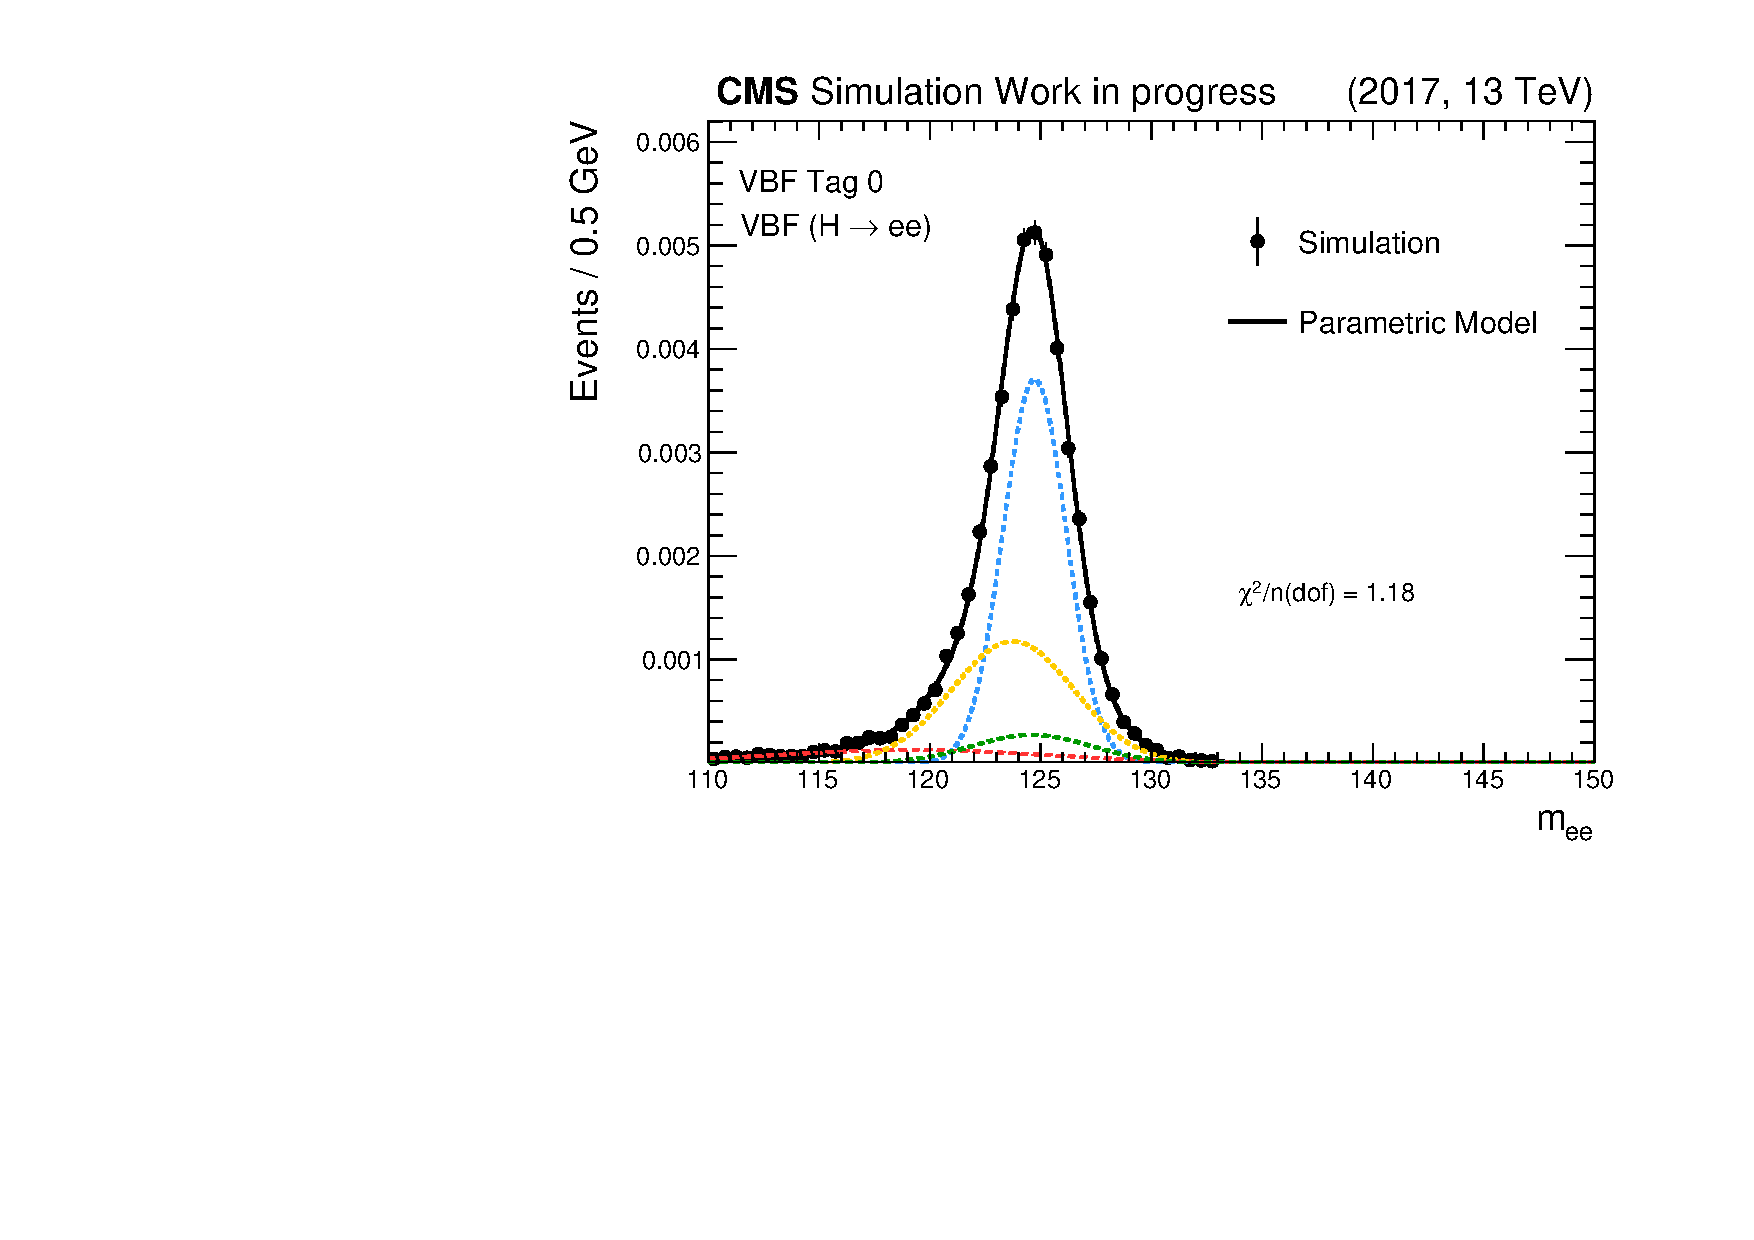
\includegraphics[width =0.49\linewidth]{Figures/Hee/Results/sigModels/GaussSums/total_shape_pdf_components_VBF_vbfcat0.pdf}
\caption[Components of the signal model for the \ggH Tag 0 and VBF Tag 0 analysis categories.]{Shape components of the \mee signal model for simulated \ggH events in the most pure ggH analysis category (left), and simulated VBF events in the most pure analysis category targeting VBF events (right). Events are shown for 2017 only, and simulated assuming \mH= 125~GeV. Contributions from up to five Gaussian functions are shown by the dashed lines, with the FSR Gaussian displayed in red. The overall model, resulting from the sum of each Gaussian distribution, is shown by the solid black line.}
\label{fig:smode_components}
\end{figure}

To allow for the extraction of limits on \BHee as a function of the Higgs boson mass, signal models are constructed from a simultaneous fit to samples at \mH= 120, 125, and 130~GeV. Each parameter for each Gaussian is a linear function of \mH,  which accounts for the dependence of the signal model shape on the Higgs boson mass. 
The exact number of Gaussian probability distributions used for each model depends on the shape of the \mee distribution, and is chosen to maximise the $\chi^{2}/n_{dof}$ in the signal fit. %defined as: (n_m(ee)_bins - no free params in function); therefore prevents overfitting

For each value of \mH, the total signal yield for each production process is normalised by the product of the cross section times branching fraction for the \Hee decay. For intermediate mass hypotheses, this normalisation is extracted using a spline constructed from piece-wise polynomial functions, through the three original \mH values. Each yield is also normalised to the product of the detector efficiency and analysis acceptance, defined by the ratio of the number of events entering the overall analysis category acceptance, to the total number of expected events. To illustrate the evolution of signal models with \mH, Figure~\ref{fig:sModels_vs_mh} shows example models at a selection of Higgs boson mass hypotheses, for ggH signal entering in the highest $S/B$ category targeting \ggH events, in 2016 simulation. The signal normalisation is also shown, divided into its constituent components.

\begin{figure}[htbp!]
\centering
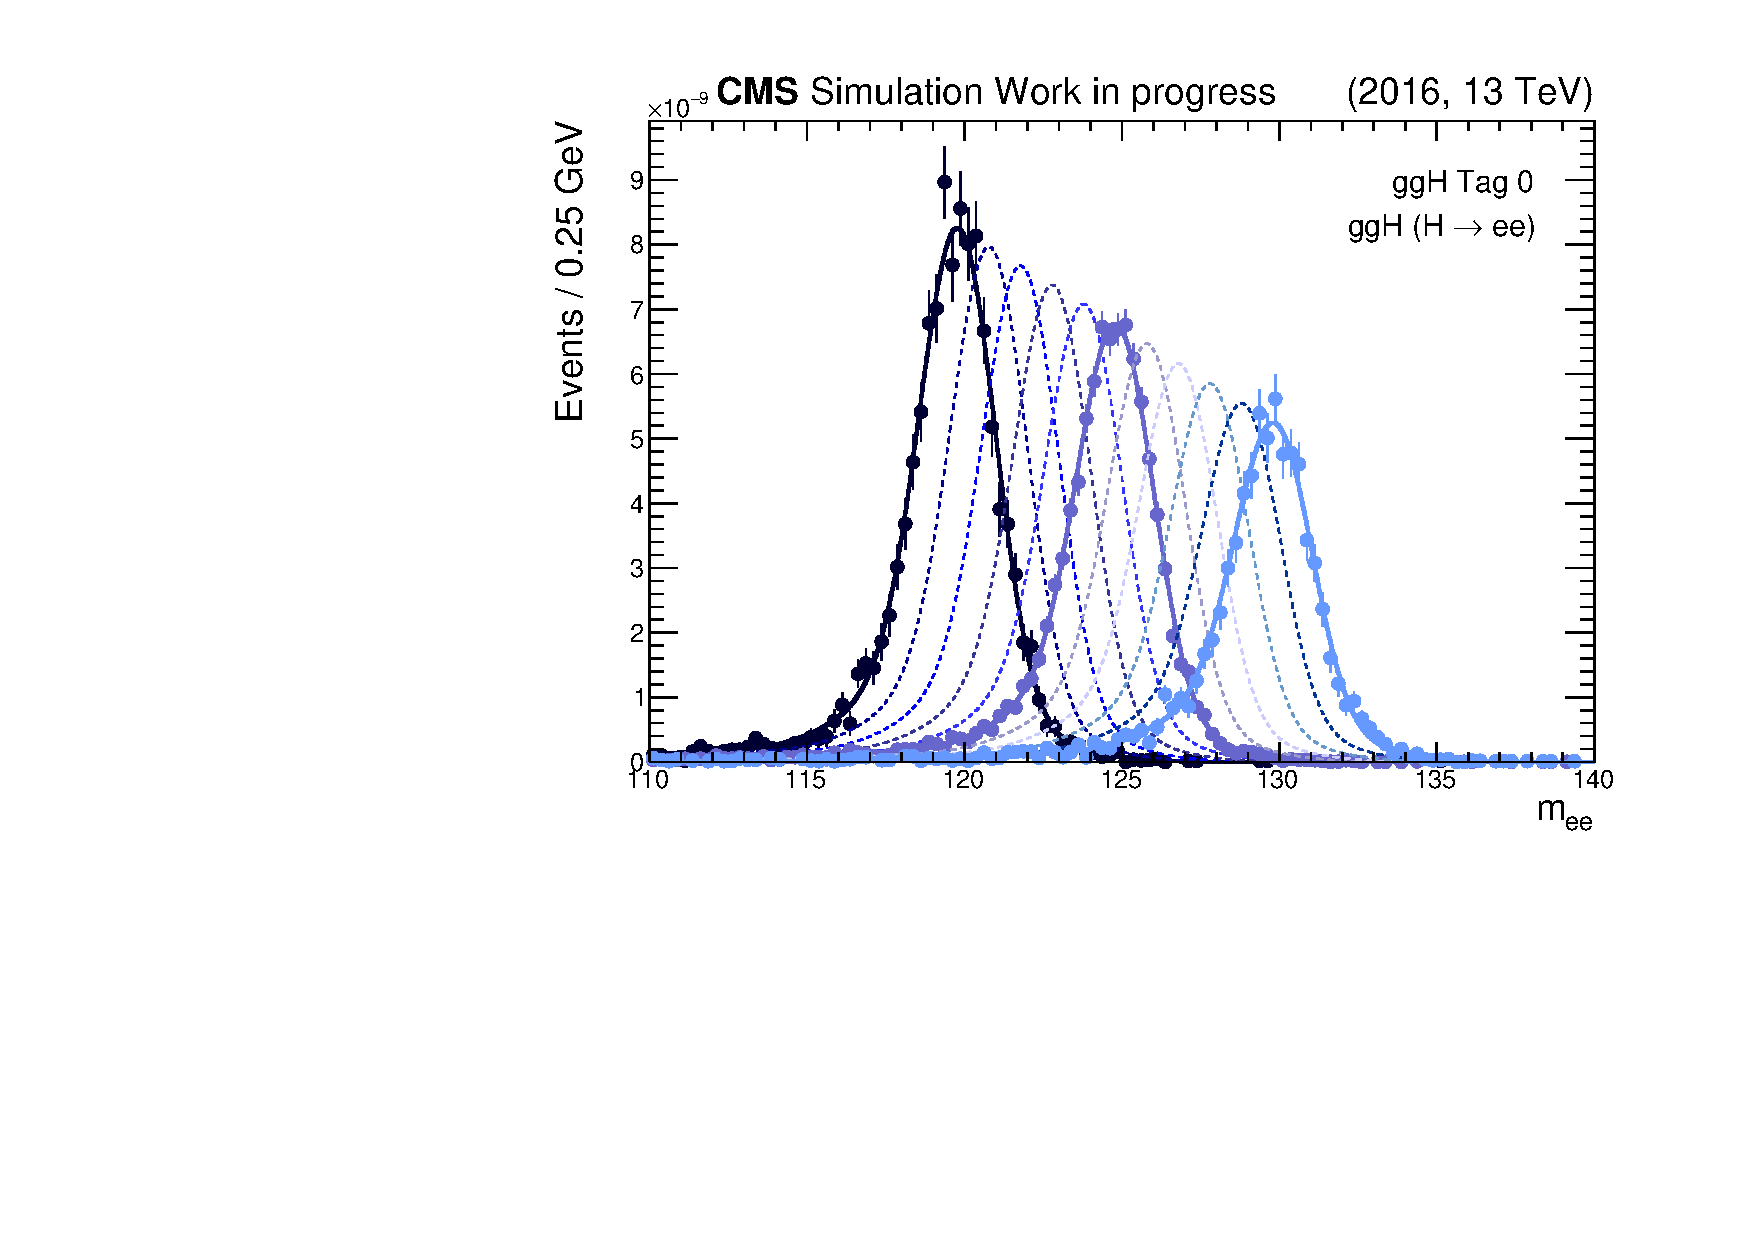
\includegraphics[width =0.49\linewidth]{Figures/Hee/Results/sigModels/modelVsMHExample/GG2H_2016_gghcat0_13TeV_model_vs_mH.pdf}
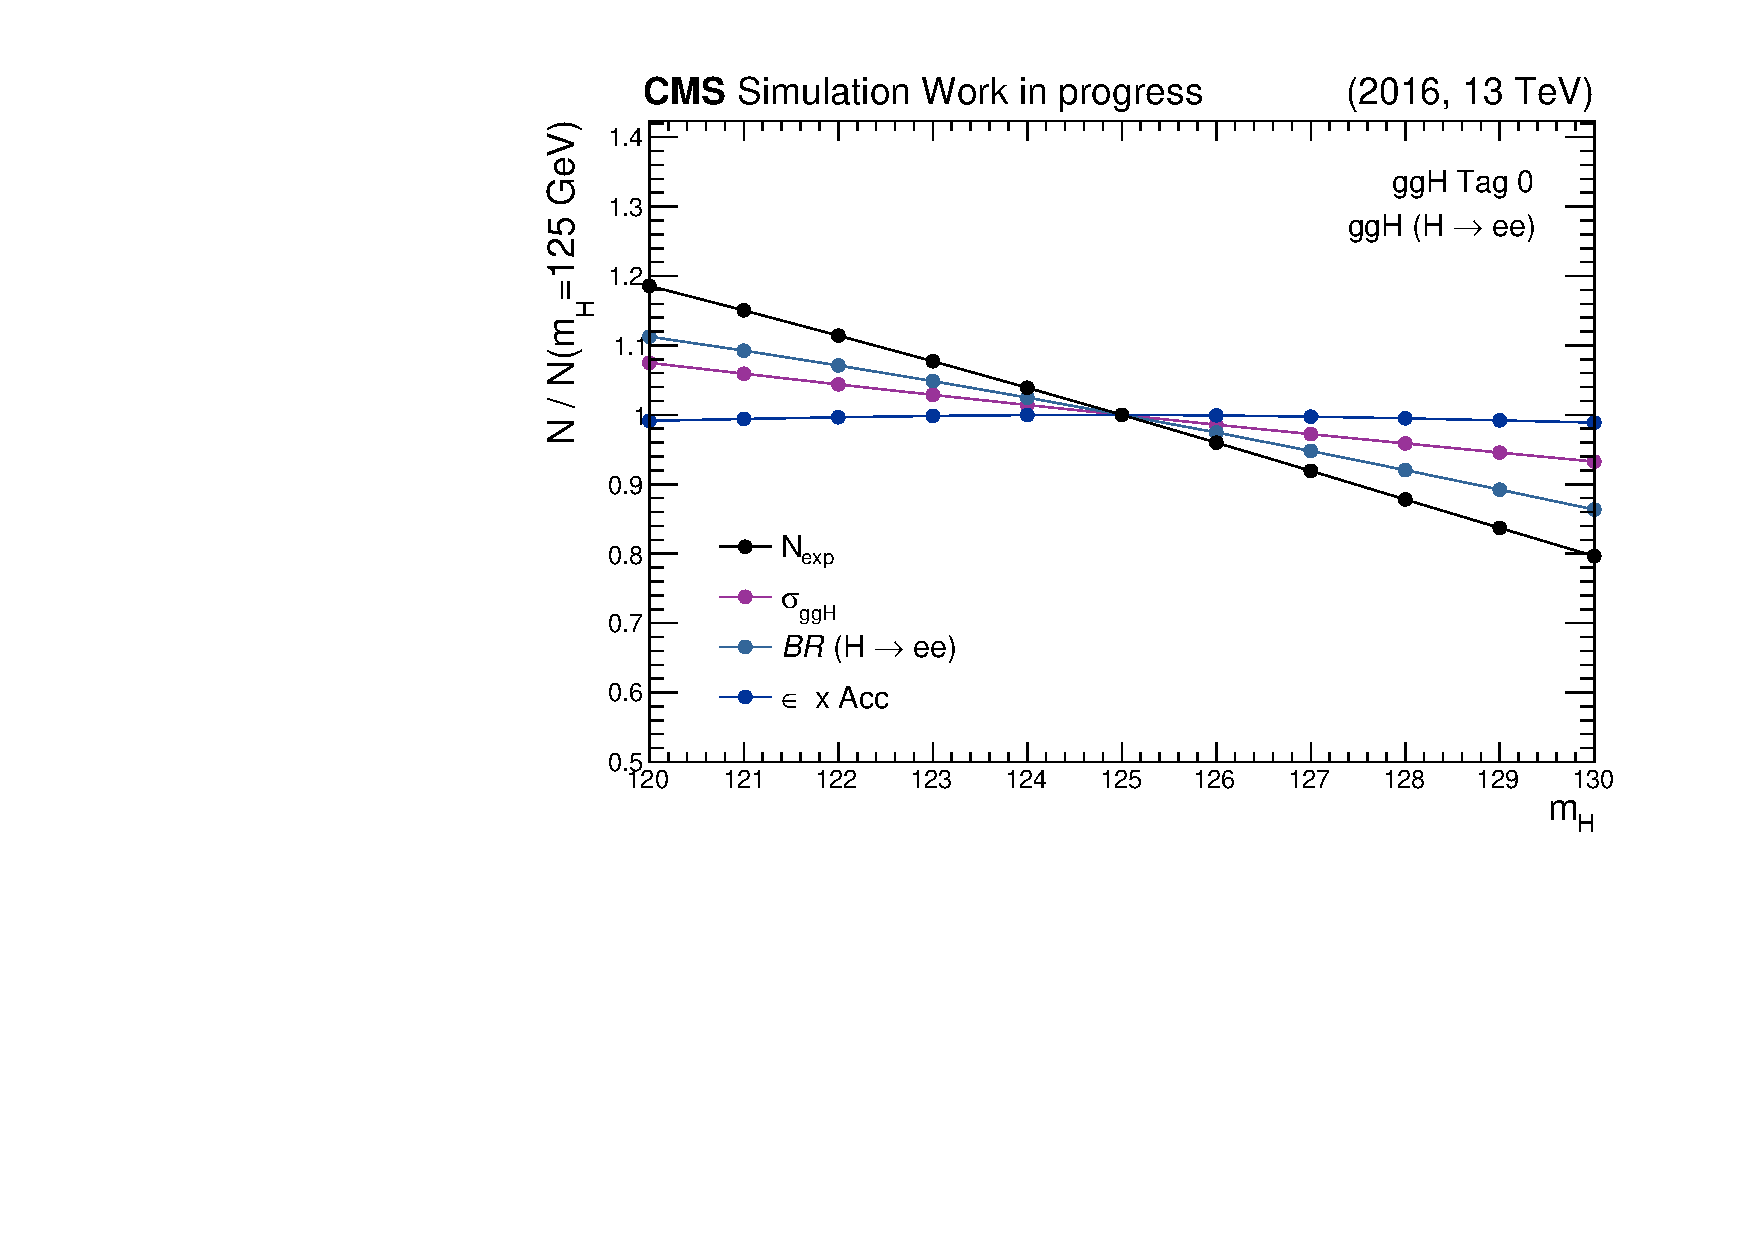
\includegraphics[width =0.49\linewidth]{Figures/Hee/Results/sigModels/modelVsMHExample/GG2H_2016_gghcat0_13TeV_splines.pdf}
\caption[The signal model for \ggH events in the ggH Tag 0 analysis category, in 2016, as a function of the Higgs boson mass, alongside the signal normalisation.]{Left: the evolution of signal models with \mH, for simulated \ggH signal events in ggH Tag 0, in 2016. Simulated events for Higgs boson masses of \mH= 120, 125, and 130~GeV are shown, along with their statistical uncertainty, by the filled markers. Dashed lines indicate signal models for intermediate Higgs boson mass hypotheses. Right: normalisation of the signal yield for the same simulated events, as a function of \mH, scaled to the nominal yield at \mH= 125~GeV. The overall normalisation is broken into contributions from the production cross section, \Hee branching fraction, and the combination of the detector efficiency and analysis acceptance.}
\label{fig:sModels_vs_mh}
\end{figure}

%The total signal yield for each production process is normalised by the product of the cross section times branching ratio for \Hee, computed using the current best measurement of the Higgs boson mass from the CMS experiment, $\mH=125.38$~GeV\cite{CMS_Hgg_Hmass}. Since the simulated signal is generated assuming a nominal Higgs boson mass of 125.0~GeV, the normalisation step firstly requires shifting the mean of each signal model by 0.38~GeV. The \mee resolution is assumed to remain unchanged, an assumption that is valid provided the difference in resolution between mass points is covered by the systematic uncertainties introduced in Section~{\ref{subsec:hee_syst_uncertainties}}. The yields are also normalised to the product of the detector efficiency and analysis acceptance, defined by the ratio of events entering the overall analysis category acceptance compared to the total number of expected events. %this relies on the assumption that the eff and acc does not change considerably between the two mass points

Figure~\ref{fig:hee_smodels} shows the final signal models for the highest $S/B$ analysis categories targeting \ggH and VBF events, for a nominal Higgs boson mass of \mH= 125~GeV. 

\begin{figure}[htbp!]
\centering
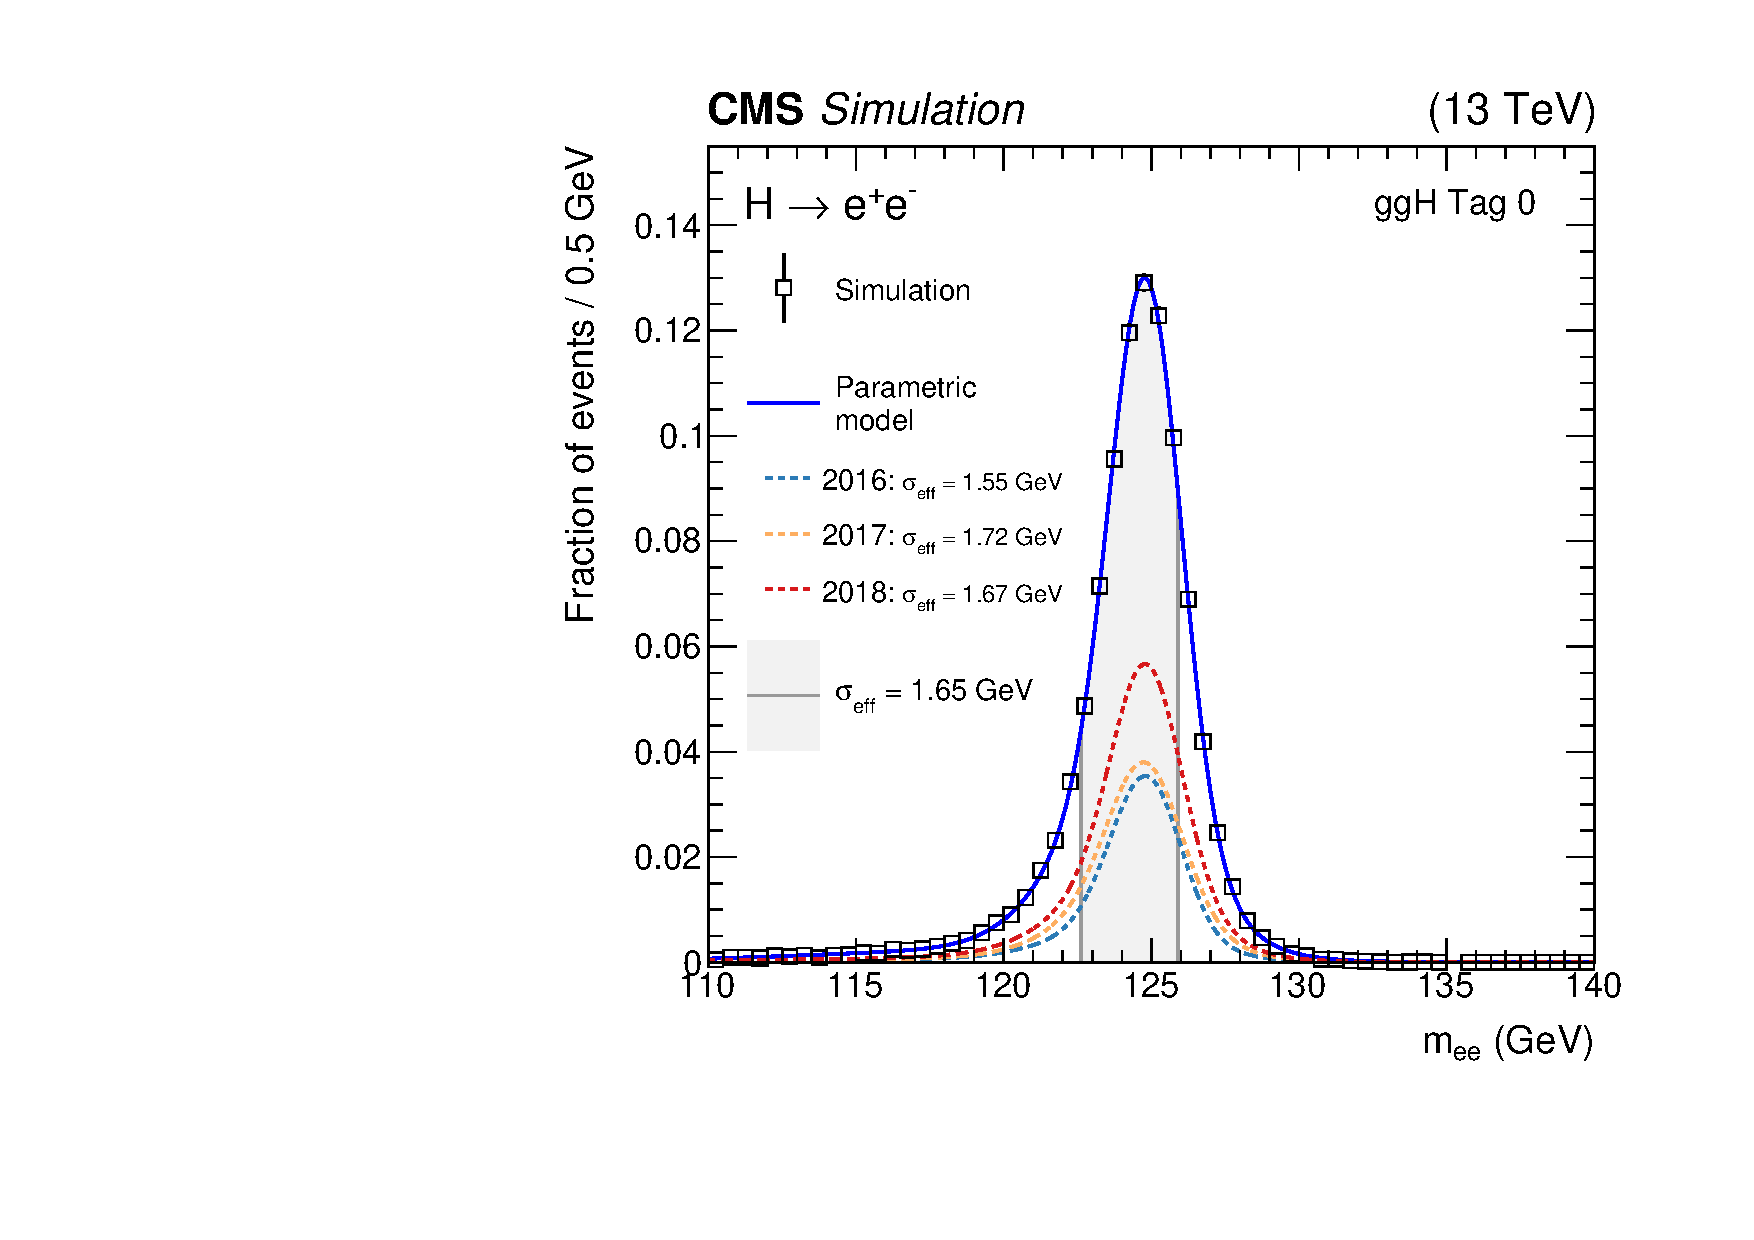
\includegraphics[width =0.48\linewidth]{Figures/Hee/Results/sigModels/nominal/smodel_gghcat0_paper.pdf}
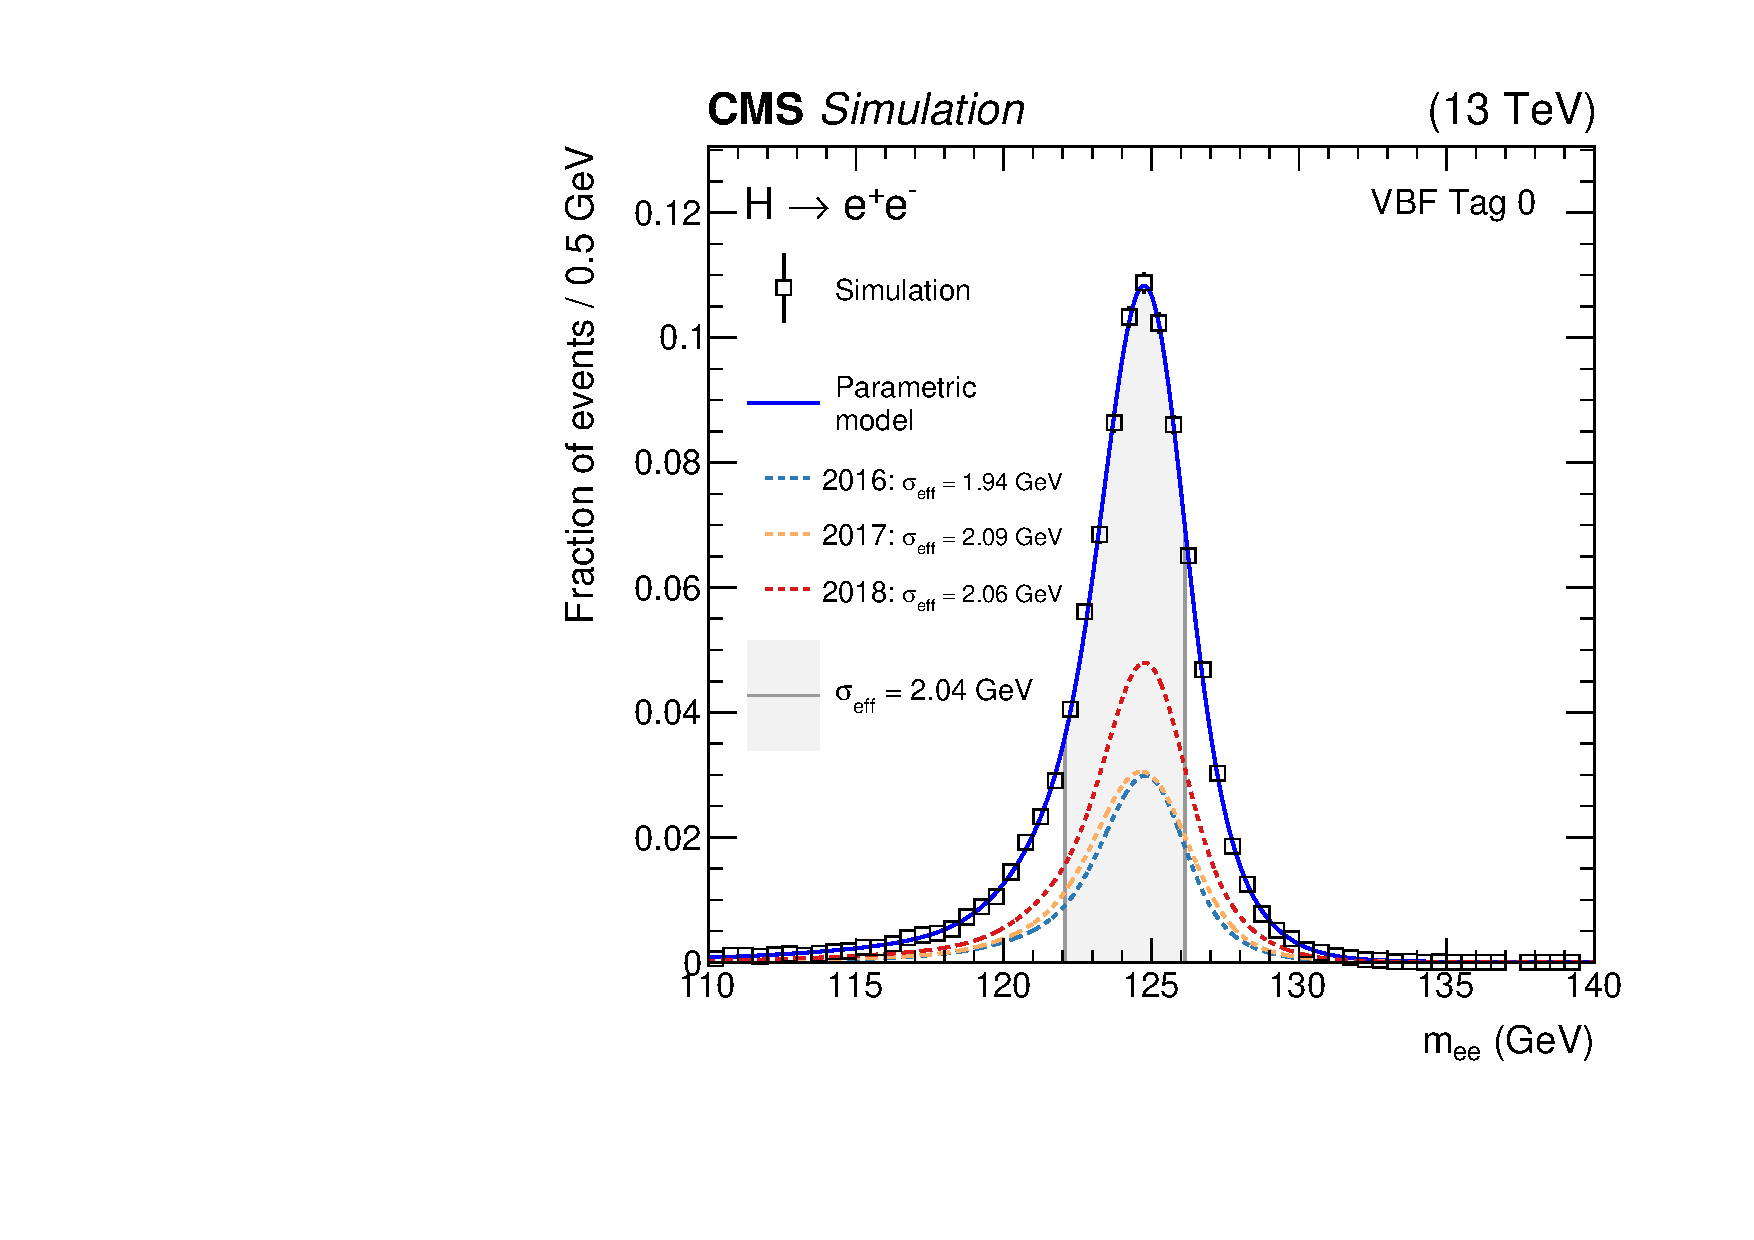
\includegraphics[width =0.48\linewidth]{Figures/Hee/Results/sigModels/nominal/smodel_vbfcat0_paper.pdf}
\caption[The signal model for the \ggH Tag 0 and VBF Tag 0 analysis categories.]{Signal models for the two highest $S/B$ analysis categories targeting \ggH (left) and VBF (right) production, integrated over Higgs boson production processes, for a nominal Higgs boson mass of \mH= 125~GeV. The overall yield is normalised such that the integral is equal to unity. The contribution from each of the three years is shown by the dashed lines. The resolution, parameterised using \seff, is also labelled for each model.}
\label{fig:hee_smodels}
\end{figure}

\section{Background modelling}
\label{subsec:hee_b_modelling}

Background events in the \Hee search comprise those entering analysis categories that originate from processes other than the \Hee signal. These events, predominantly originating from DY decays, form a smoothly falling distribution in \mee, on top of which the signal peak is situated. Unlike in the construction of signal models, an entirely data-driven approach is used to model the background. The strategy uses data in the sideband region, defined as data outside $115<\mee<135$~GeV, to constrain functional forms for the background models. This offers the advantage that any systematic effects associated with the modelling and reconstruction of simulated background samples is avoided.

The exact parameterisation of the background distributions are not known a priori, and thus many functional forms that fit well are considered. This degeneracy in the parameterisation translates into an uncertainty on any measurements of the signal, since each choice of function results in a different number of events counted under the signal peak. To account for this uncertainty, the discrete profiling method is used, described in detail in Ref~\cite{envelope_method}. This reference includes tests of the coverage for the method, and bias on the extracted parameters of interest (POIs), the latter of which is also tested explicitly in Section~\ref{subsec:hee_bias_studies}.

To introduce the discrete profiling method, it is useful to outline the concept of nuisance parameters, and their effect on the NLL curve. In general, a nuisance parameter is any parameter of a model which affects the parameters of interest, but is not of interest itself. When fitting for the POIs, the nuisance parameter is profiled, meaning its value is allowed to vary during the minimisation of the likelihood, potentially within some constraint. This is illustrated in Figure~\ref{fig:hee_disc_prof_plot}, where the blue curve shows the negative logarithm of the likelihood, for some parameter of interest, $\mu$, when the nuisance parameters are fully profiled. 
If the nuisances were fixed to their best fit values, as illustrated in the orange parabola, the likelihood curve would be narrower, and the uncertainty interval on $\mu$, smaller.
However, when profiling the nuisance parameters, a configuration can can be found for each point in $\mu$-space that decreases the NLL (increases the likelihood). Smaller values for the NLL result in the likelihood curve tracing a wider parabola, naturally increasing the measured uncertainty on $\mu$.

Although the above example describes a continuous profiled nuisance, the same curve could be built by ensembling a set of negative log-likelihood curves where nuisance parameters can take on discrete values. In the example of Figure~\ref{fig:hee_disc_prof_plot}, curves generated by arbitrary values of the nuisance parameters are shown in red. Although a discrete number of these are drawn, the entire profile likelihood curve could be constructed from the envelope enclosing all such red curves, provided the nuisance parameter space is sampled sufficiently. %i.e. envelope each indivudal curve built by looking at a given value for mu, and setting the nuisances the values corresponding to the best-fit i.e. lowest point in the individual likelihood curve. So this is like ensembling the best fits at all points in the POI space. NOTE that plot is kind of the other way around - we sample different points in the nuisance parameter space, and get the best fit mu for each one. If we sample enough nuisances, we build up the full curve where the nuisances are profiled/floating
This equivalent formalisation demonstrates the generalisation between a discrete and continuous set of nuisance parameters.

\begin{figure}[htbp!]
\centering
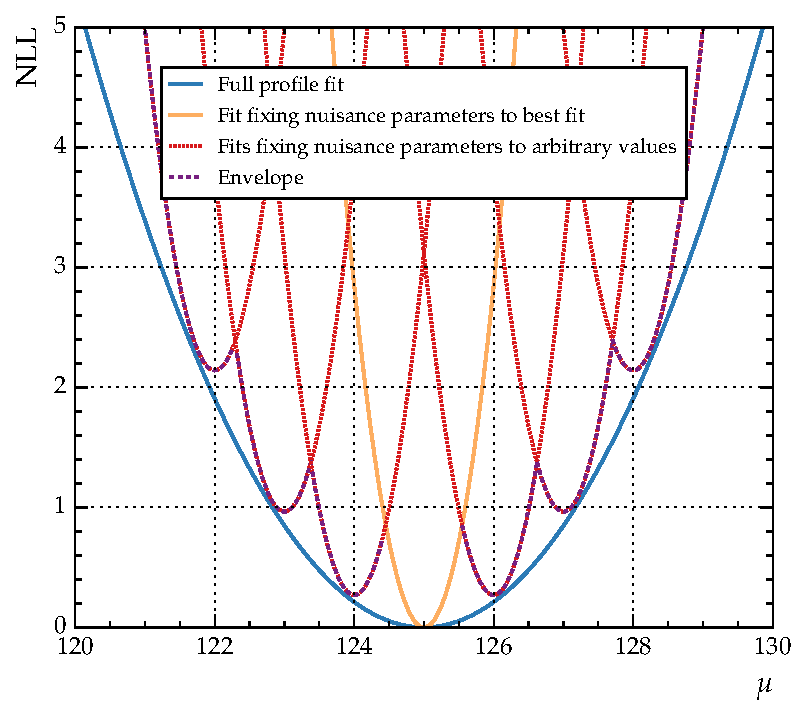
\includegraphics[width =0.6\linewidth]{Figures/Hee/Results/bkgModels/DPM.pdf}\hfill%
\caption[An illustration of the discrete profiling method.]{An illustration of the discrete profiling method. The negative log-likelihood curve, where the set of nuisance parameters are allowed to vary at each value of the POI, $\mu$, is shown in the solid blue line. The fully profiled curve can be built from the envelope (dashed purple line) of curves generated at discrete configurations of the nuisance parameter space. These  curves, shown in red, are produced by nuisances fixed at arbitrary values other than those at the best fit, and approximate the fully profiled fit when the number of nuisance parameter configurations sampled is large. Figure inspired by Ref~\cite{envelope_method}.}
\label{fig:hee_disc_prof_plot}
\end{figure} 
%this is kinf of the opposite

In the case of modelling the background \mee distribution in the \Hee analysis, the choice of functional form with which to fit is treated as a discrete nuisance parameter. The resulting 2NLL envelope is then constructed by profiling all possible choices of background parameterisation.
Although in principle all analytical functions that fit the background \mee distribution well could be tested, in practise, the chosen parameterisations can be divided into two groups of functional families. The first set consists of functions that are able to describe, in principle, smoothly falling distributions, given an appropriate choice for the number of degrees of freedom. Four families are considered in this group; for a $N$-parameter function with parameters $p_0, p_1, ..., p_N$ to be determined, these include:
 
\begin{itemize}
\item sum of exponential functions, where
\begin{equation*}
f_N(\mee) = \sum_{i=0}^{N} p_{2i}\exp{\left(p_{2i+1}\cdot\mee\right)},
\end{equation*}
\item sum of power law functions, where
\begin{equation*}
f_N(\mee) = \sum_{i=0}^{N} p_{2i}\cdot\mee^{-p_{2i+1}},
\end{equation*}
\item Bernstein polynomials, where
\begin{equation*}
f_N(\mee) = \sum_{i=0}^{N} p_{i}\binom{N}{i}\mee^{i}\left(1-\mee\right)^{N-i},
\end{equation*} and
\item Laurent series, where
\begin{equation*}
f_N(\mee) = \sum_{i=0}^{N} p_{i}\cdot\mee^{-4 + L(i)},
\end{equation*}
with
\begin{equation*}
L(i) = \sum_{j=0}^{i}(-1)^j j .
\end{equation*}
\end{itemize}

\noindent Since the expected background in all analysis categories is composed primarily of DY events, the second set of functions are included to model this smoothly falling distribution, driven by the Breit-Wigner nature of the $\mathrm{Z}$ boson lineshape. Three individual functions are considered, characterised by a core Breit-Winger component, modified by exponential or power law terms. This set of so-called physics-inspired functions include:

\begin{itemize}
\item Breit-Wigner core modified by an exponential function of \mee, where
\begin{equation*}
f_N(\mee) = \frac{\Gamma_{Z}\cdot\exp(p_{0}\cdot\mee)}{(\mee - m_{Z})^{2} + (\Gamma_{Z}/2)^{2}},
\end{equation*}
\item Breit-Wigner Redux, where the Breit-Wigner core is modified by a further exponential term, and the exponent in the denominator becomes a free parameter, where
\begin{equation*}
f_N(\mee) = \frac{\Gamma_{Z}\cdot\exp(p_{0}\cdot\mee + p_{1}\cdot\mee^{2})}{(\mee - m_{Z})^{p_{2}} + (\Gamma_{Z}/2)^{p_{2}}},
\end{equation*}
\item Breit-Wigner Gamma, where a Breit Wigner, modified by a single exponential factor, is summed with a gamma function, where
\begin{equation*}
f_N(\mee) = p_{2}\cdot\frac{\Gamma_{Z}\cdot\exp(p_{0}\cdot\mee)}{(\mee - m_{Z})^{2} + (\Gamma_{Z}/2)^{2}} + (1-p_{2})\cdot\frac{\exp{(p_{1}\cdot\mee)}}{\mee^{2}}.
\end{equation*}
\end{itemize}

\noindent For efficiency, the final envelope of candidate functions considers only a subset of the possible choices. The procedure to select functions is performed separately for each analysis category, and proceeds as follows. The lowest order functions in the family are fit, using a maximum likelihood approach, to the \mee sideband regions in data. The process is repeated for subsequent orders of the function, until a minimum requirement on the goodness-of-fit is reached. This criteria ensures that only functions fitting the \mee distribution well are included in the final category envelopes. For functions defined at a fixed order, namely the set of physics-inspired functions, the procedure is complete. For parameterisations that span multiple orders, an F-test~\cite{f_test} is then performed to quantify whether the improvement in fit quality when considering the next highest order function justifies the increase in model complexity. The test computes a $p$-value by determining the difference in 2NLL between fits of successive order as a test statistic. Assuming sufficient sample size, the statistic follows a $\chi^{2}$ distribution with degrees of freedom equal to the difference in number of parameters between the two functions under test. If the observed $p$-value is below a threshold of 0.05, the higher order function is deemed to offer a worthwhile improvement in fit quality, and is added to the category envelope. The process is repeated for each successive order until the $p$-value requirement is failed.  % i guess distributed as a chi squared under the hypothesis that the increase in DOF does not alter the fit (quality)??
To further prevent overfitting, an additional penalty term is applied to penalise overly complex functions. The penalty adds one unit to the negative log-likelihood for each free parameter in the background model and is applied in the final signal-plus-background fit.

Figure~\ref{fig:hee_bmodels} shows all functions entering the envelope for the highest $S/B$ analysis categories targeting \ggH and VBF events. The degeneracy in possible fits is well spanned by the set of candidate functions. The envelope in each category consists of roughly equal numbers of physics-inspired and nominal smoothly falling functions; the best fitting functions in each category, defined as those with the smallest NLL value amongst possible background candidates, are also equally divided between these two sets.

\begin{figure}[htbp!]
\centering
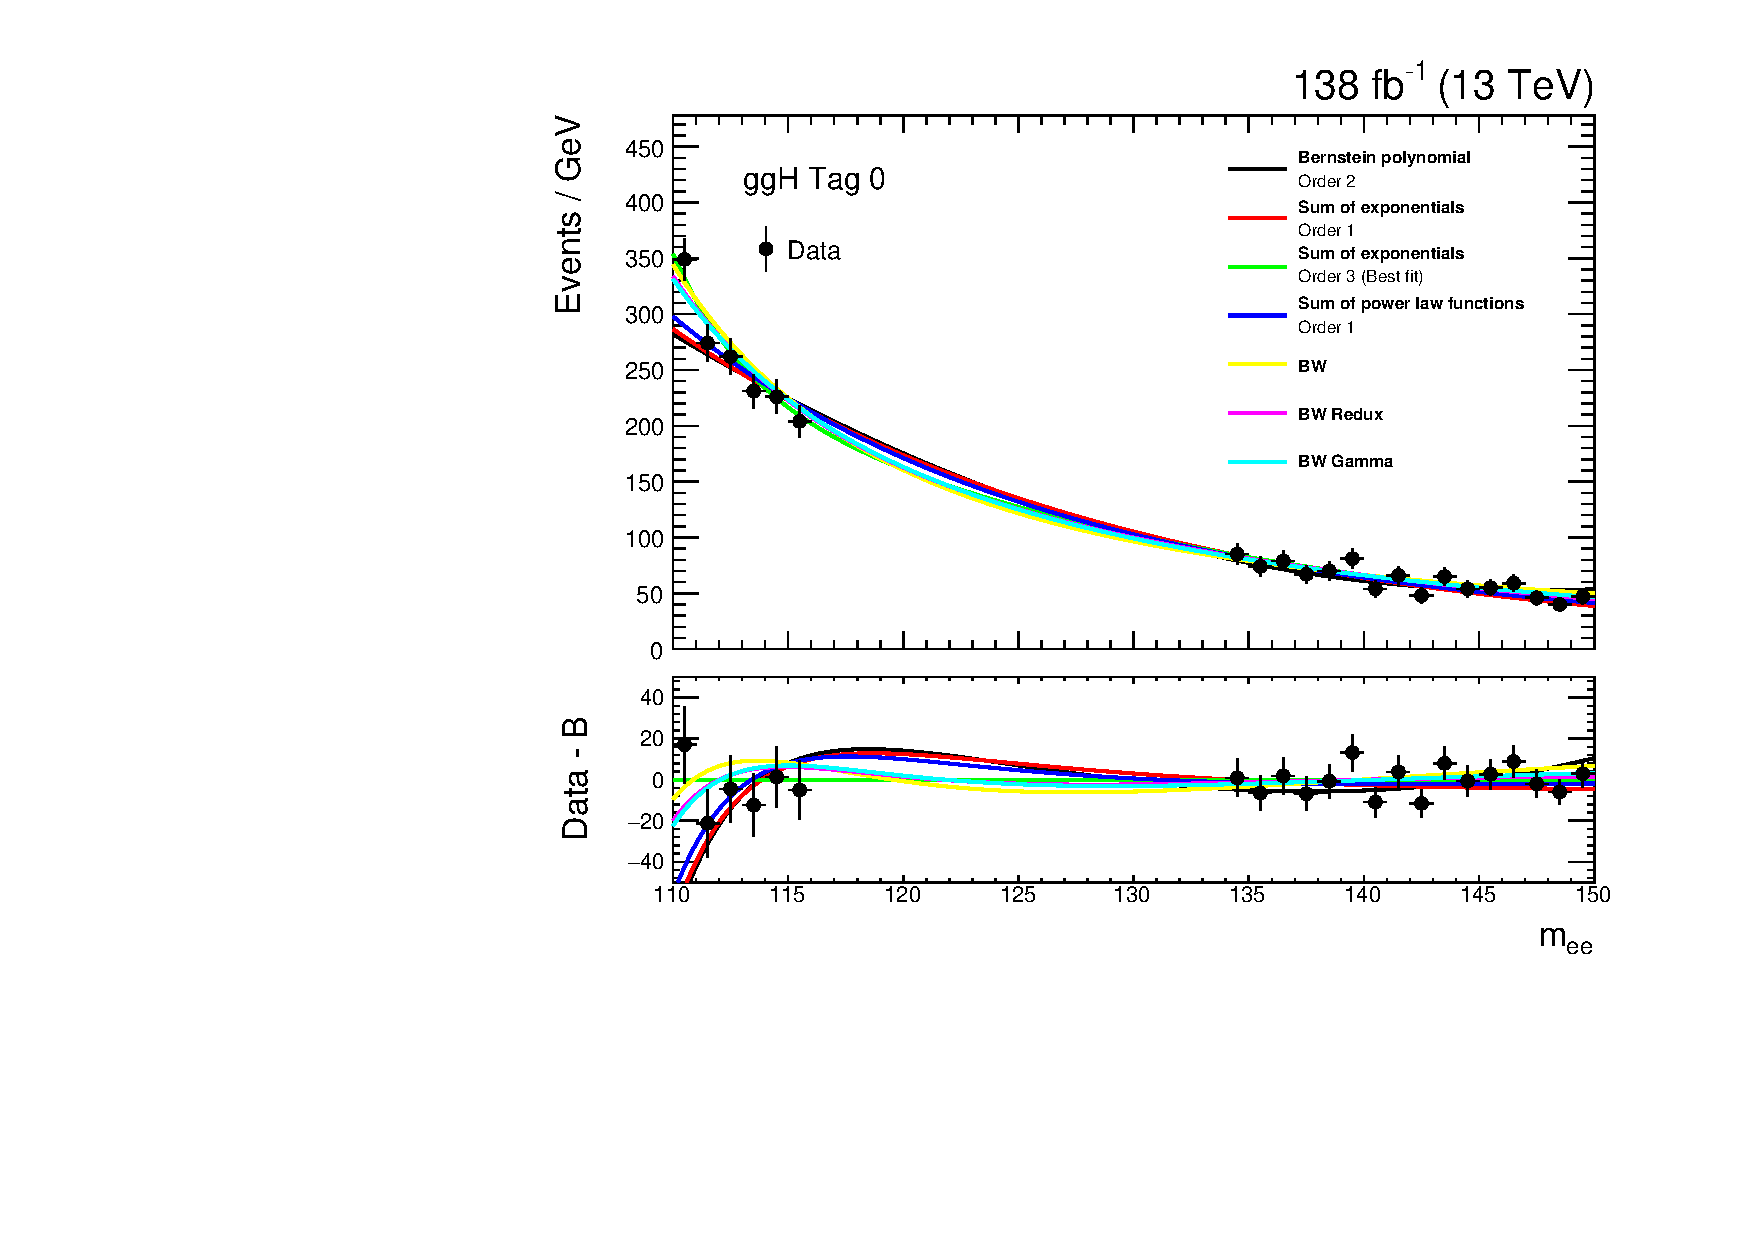
\includegraphics[trim={0cm 3.5cm 0cm 0cm},clip,width =0.495\linewidth]{Figures/Hee/Results/bkgModels/bmodel_gghcat0.pdf}
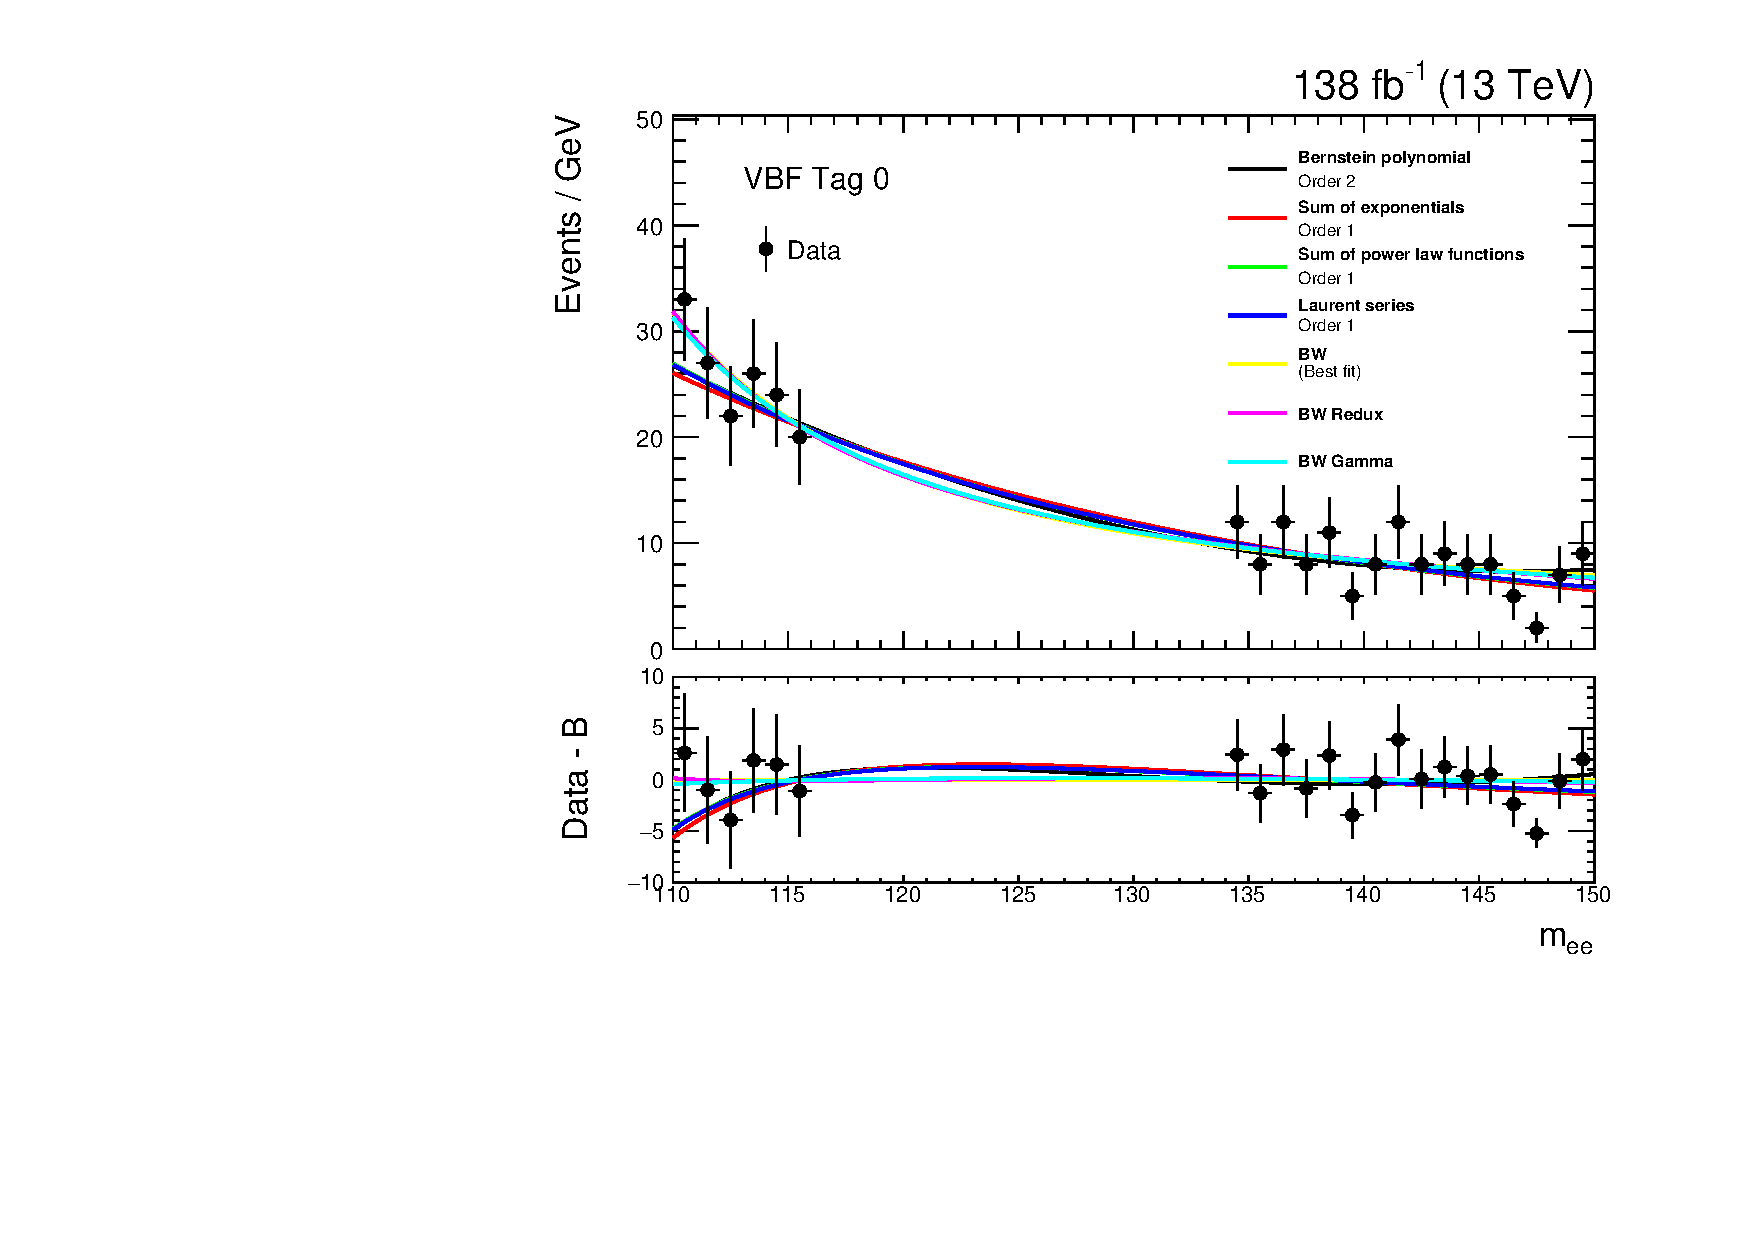
\includegraphics[trim={0cm 3.5cm 0cm 0cm},clip,width =0.495\linewidth]{Figures/Hee/Results/bkgModels/bmodel_vbfcat0.pdf}
\caption[The set of candidate background functions for the \ggH Tag 0 and VBF Tag 0 analysis categories.]{The set of candidate functions chosen to fit data in the \mee sideband regions using the envelope method, for the highest $S/B$ category targeting \ggH (left) and VBF (right) events. The functional families considered include sums of exponential functions, Bernstein polynomials, sums of power law functions, and Laurent Series', as well as modified Breit-Wigner functions aiming to model the lower tail in \mee resulting from $\mathrm{Z}$ boson decays. The best fitting function is indicated in the legend. The residual difference between each background model and data is shown in the lower panel. }
\label{fig:hee_bmodels}
\end{figure}

Finally, the background resulting from SM \Hgg production, where both photons are misreconstructed as electrons, is studied with simulated events. The process is found to contribute less than 0.1\% to the inclusive analysis categories, for a \Hee branching fraction scaled to the expected limit obtained in chapter~\ref{chap:results}. It is therefore neglected in the rest of the analysis.


\subsection{Bias studies}
\label{subsec:hee_bias_studies}

Although many parameterisations of the background \mee distribution are considered for each value of the POI, in the end, only one function minimising the likelihood is chosen. Therefore, it is possible that this choice of function may inject a systematic bias on the extracted \Hee branching fraction. To check for possible bias, a large sample of pseudo-experiments, or \textit{toys}, are generated using a Monte Carlo technique. Toy datasets are built for the \mee distribution in all analysis categories from each of the candidate background functions in the envelope. The function used to generate the background \mee distribution is considered as the ``true" background parameterisation for the given set of toys. Each toy also is also injected with a signal proportional to the expected limit on \BHee, assuming a Higgs boson mass of 125~GeV. For each true background function, two thousand generated toys are fit using the discrete profiling method with the full envelope of functions included in the analysis category. 

The bias for each toy dataset is defined using the pull of the distribution, where the pull for a given toy is

\begin{equation}\label{eqn:hee_bias}
    P(\mu,\hat{\sigma}) = \frac{\hat{\mu}-\mu}{\hat{\sigma}},
\end{equation}



\noindent where $\mu$ is the injected value of the rate parameter scaling \BHee, $\hat{\mu}$ is the value of $\mu$ which minimises the NLL for each toy, as returned from the fit, and $\hat{\sigma}$ is the uncertainty on $\hat{\mu}$. In the absence of systematic effects, the pull over all toys is expected to be Gaussian distributed, with a mean of zero and standard deviation of one. Practically, a Gaussian function is fit to the pull distribution, with the mean of the fit being used to quote the bias.  
Good functional forms are those characterised by an absolute bias of less than 0.2, where this threshold is chosen to ensure that the systematic uncertainty due to a potential bias on the upper limit for \BHee does not increase the overall uncertainty by more than 2\%.

The biases for the highest $S/B$ analysis categories targeting \ggH and VBF events are summarised in Figure~\ref{fig:hee_per_category_pulls}.
For almost all truth functions across each analysis category, the bias is within the accepted tolerance.
It is also checked from toys that those functions which are outside the acceptable bias range 
are rarely the best-fit choice from the envelope in each category.

\begin{figure}[htbp!]
\centering
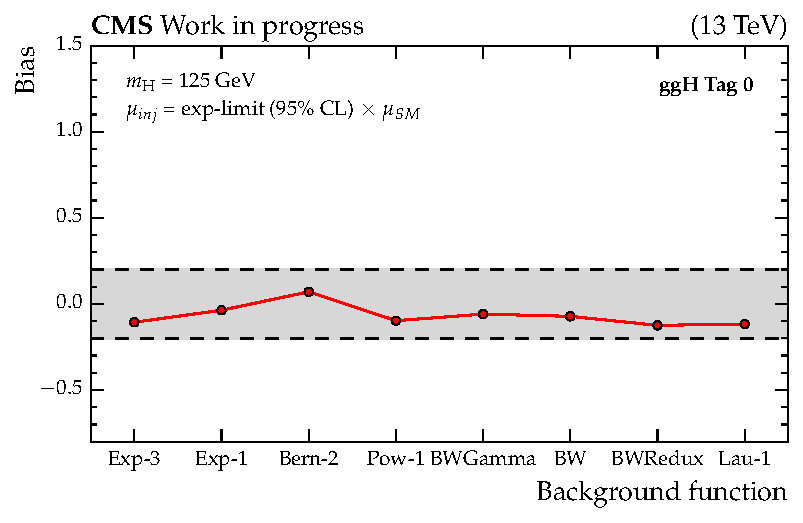
\includegraphics[width =0.49\linewidth]{Figures/Hee/Results/biasStudies/pulls_gghcat0.pdf}
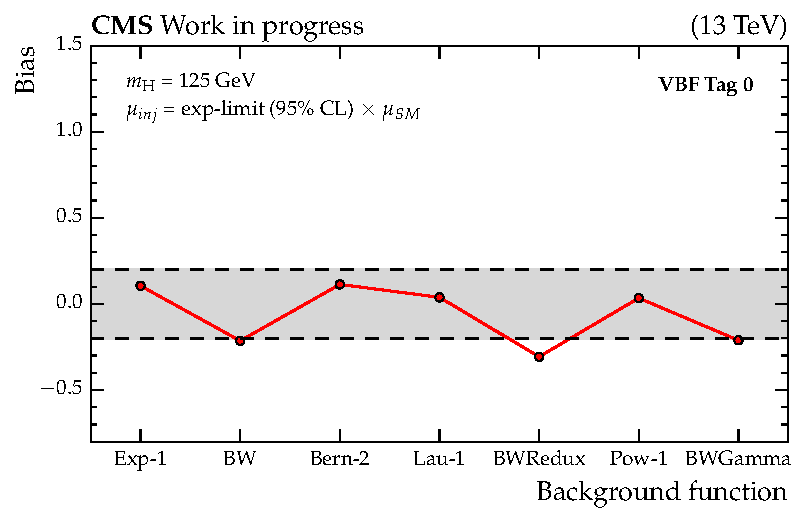
\includegraphics[width =0.49\linewidth]{Figures/Hee/Results/biasStudies/pulls_vbfcat0.pdf}
\caption[The bias for each background candidate function in the envelope for the \ggH Tag 0 and VBF Tag 0 analysis categories.]{The measured bias of each ``true" function inside the envelope of possible background fits used to generate toy datasets, for the highest $S/B$ analysis categories targeting \ggH (left) and VBF (right) events. Each toy dataset is injected with a signal model with yield scaled to the expected limit on \BHee, assuming a nominal Higgs boson mass of 125~GeV. The individual functions and their order are specified along the $x$-axis. For almost all functions, the bias is within the chosen tolerance of $\pm0.2$ (grey shaded-band).}
\label{fig:hee_per_category_pulls}                                                                                 
\end{figure}


\section{Systematic uncertainties}
\label{subsec:hee_syst_uncertainties}

Unlike the data-driven background models, where systematic uncertainties are handled naturally using the discrete profiling method, uncertainties affecting the signal models must be estimated directly from simulation. These uncertainties are treated in one of two ways. Uncertainties which could modify the shape of the \mee distribution are incorporated as Gaussian constrained nuisance parameters that modify the mean and width of the signal distributions in each analysis category. %The constraint term adds a penalty to the likelihood when a nuisance parameter is fit away from its mean value, to prevent unphysical systematic shifts. Nick removed this since its really just meant to model prior information about the observable i.e. the value is distributed as a gaussian
Variations that modify the signal shape typically arise from uncertainties in the electron energy scale calibration. Uncertainties that do not affect the \mee shape are treated as log-normal variations in the signal yield. These are allowed to modify the normalisation in both directions asymmetrically, although each variation is typically comparable in magnitude. Systematic uncertainties that affect only the signal yields typically arise from theoretical sources associated with the simulation of signal events, and experimental uncertainties describing, for example, the electron reconstruction and identification efficiencies.

\subsection{Theoretical uncertainties} 

The sources of theoretical uncertainty considered in this analysis are as follows.
   
%there is no dedicated eff-acc uncertainty, we assuming it cancels in the ratio of measured/SM stuff. But it can change by other systs e.g. JEC can introduce category migrations.
%we also need XS theory uncertainties because we are assuming SM cross sections which (which we dont do in the STXS analysis since we float this)   
  
\begin{itemize}
\item \textit{QCD scale uncertainty}:  
  the uncertainty arising from variations of the renormalisation and factorisation scales used when computing expected SM cross sections and event kinematics.
  These account for the missing higher order terms in perturbative calculations.
  The recommendations provided in Ref~\cite{YR4} are followed, where the uncertainty in the yield is estimated using three sources: varying the renormalisation scale by a factor of two, varying the factorisation scale by a factor of two, and varying both in the same direction simultaneously.
  The impact on the normalisation is largest for \ttH events at 5.8\%. %Includes over uncertainties on the cross section that can change the norm, and then migration uncertainties that can e.g. scale individual categories ggH3 down and ggH0 up if says the QCD scale made events have a higher pT. But note we dont hand pick events and place into categories, we just have a rate param for each category that can scale events already in them (which is an approximation!).
\item \textit{PDF uncertainties}:
  these account for the uncertainty due to imperfect knowledge of the composition of the proton, which affects which partons are most likely to initiate high energy events.
  Uncertainties are computed following the PDF4LHC prescription~\cite{PDF4LHC,YR3}, with the impact on the normalisation ranging between 1.9 and 3\%.
\item \textit{Uncertainty in the strong force coupling constant}:
  the uncertainty in the value of the strong force coupling constant is included in the treatment of the parton density function uncertainties.
  The impact on the yield is largest for \ggH production, with a value of 2.6\%.
\item \textit{Underlying event and parton shower uncertainties}:
  these uncertainties are obtained using dedicated simulated samples which vary the \textsc{Pythia8} tune from that used in the nominal samples, and vary the renormalisation scale for QCD emissions in initial state and final state radiation by a factor of 2 and 0.5. These uncertainties are treated as migrations of events from a given production mode into and out of the VBF and ggH analysis categories. The largest effect comes from the parton shower uncertainty on VBF events, which can change the signal yield in the VBF analysis categories by up to 5\%. 
\end{itemize}

\noindent The total impact on the \BHee measurement from theoretical systematic uncertainties is ${}^{+0.2}_{-0.1} \times 10^{-4}$, with dominant contributions from uncertainties affecting the \ggH production cross section.

\subsection{Experimental uncertainties}

Experimental uncertainties that affect the shape of the \mee distribution in signal events are listed below.
   
\begin{itemize}
\item \textit{Electron energy scale}:
  the uncertainty associated with the corrections applied to the electron energy scale in simulation~\cite{CMS_egamma_performance}, derived using a sample of \Zee tag-and-probe events~\cite{TagAndProbe}. Four nuisance parameters are defined for the possible combinations of electrons with low or high $R_{9}$ values, and reconstructed within the EE or EB. %what about the corrections to data? do they have systs?
\item \textit{Electron energy scale non-linearity}:
  an uncertainty to cover possible differences between the linearity of the electron energy scale between data and simulation, estimated on a sample of boosted tag-and-probe events. An uncertainty of 0.1\% is assigned for electrons with \pt$<80$~GeV, and 0.2\% for above.
\end{itemize}
   
\noindent Experimental uncertainties that only modify the event yield are as follows.

\begin{itemize}
\item \textit{Integrated luminosity}:
  the integrated luminosities for the 2016, 2017, and 2018 data-taking years have individual uncertainties of 1.2, 2.3, and 2.5\% respectively~\cite{CMSlumi2016,CMSlumi2017,CMSlumi2018}, while the overall uncertainty for the 2016--2018 period is 1.6\%. 
\item \textit{Electron ID and reconstruction efficiencies}:
  uncertainties on the scale factors derived to correct for differences in simulation and data for the electron ID and reconstruction efficiencies. For both sources, the size of the uncertainty is approximately 1\% in each category.
\item \textit{Jet energy scale and smearing corrections}:
  the energy scale of jets is measured using the \pt balance of jets with $\mathrm{Z}$ bosons and photons in \Zee, \Zmumu and $\gamma$+jets events, as well as the \pt balance between jets in dijet and multijet events~\cite{JetsInRun2}.
  The uncertainty in the jet energy scale is a few per-cent and depends on \pt and $\eta$.
  The size of the jet energy scale uncertainties on event yields is evaluated by varying the jet energy corrections within their uncertainties and propagating the effect to the final result. The impact on category yields is largest for those targeting VBF, and can be as high as 15\%.
\item \textit{Trigger efficiency}:
  the uncertainty on the efficiency of the trigger selection, measured with $\Zee$ events using the tag-and-probe technique. The size of the uncertainty is less than 1\%. An additional uncertainty is introduced to account for a gradual shift in the timing of the inputs to the ECAL L1 Trigger in the region at $|\eta|\; > 2.0$, which caused a specific trigger inefficiency during 2016 and 2017 data taking~\cite{CMS_L1T}. Both electrons, and to a greater extent jets, can be affected by this inefficiency.
\end{itemize} 

\noindent The total impact on the \BHee measurement from experimental systematic uncertainties is $\pm{0.2\times10^{-4}}$, with the largest contributions arising from uncertainties affecting the electron energy scale.

\section{Summary}
The maximum likelihood fit used to extract a potential \Hee signal requires modelling of both signal and background events. In this analysis, background models are developed with a data-driven approach using the discrete profiling method. This method naturally handles the uncertainty associated with choosing a function to model the \mee distribution in background events. Conversely, signal models are derived using simulated samples. The dependence on the Higgs boson mass is deliberately built into the parameters of each signal model, such that limits can be extracted as a function of \mH. Systematic uncertainties affecting signal models are handled using nuisance parameters that can modify both the shape of signal models and the overall yields. 